% CyberSecLLM: A Hybrid Mamba-Transformer Foundation Model
% for Zero-Shot Cybersecurity Threat Intelligence
% Target: IEEE Transactions on Neural Networks and Learning Systems (TNNLS)

\documentclass[journal]{IEEEtran}

% ---- Packages ----
\usepackage[utf8]{inputenc}
\usepackage[T1]{fontenc}
\usepackage{amsmath,amssymb,amsfonts}
\usepackage{algorithmic}
\usepackage{algorithm}
\usepackage{graphicx}
\usepackage{textcomp}
\usepackage{xcolor}
\usepackage{booktabs}
\usepackage{multirow}
\usepackage{subcaption}
\usepackage{hyperref}
\usepackage{cite}
\usepackage{tikz}
\usepackage{pgfplots}
\pgfplotsset{compat=1.18}
\usetikzlibrary{shapes.geometric, arrows.meta, positioning, fit, backgrounds, calc, decorations.pathreplacing}
\usepackage{balance}
\usepackage{url}
\usepackage{array}
\usepackage{nicefrac}
\usepackage{microtype}

% ---- Custom Commands ----
\newcommand{\modelname}{CyberSecLLM}
\newcommand{\benchname}{CyberSecBench}
\newcommand{\RR}{\mathbb{R}}
\newcommand{\EE}{\mathbb{E}}
\newcommand{\norm}[1]{\left\|#1\right\|}

\begin{document}

\title{CyberSecLLM: A Hybrid Mamba-Transformer Foundation Model for Zero-Shot Cybersecurity Threat Intelligence}

\author{
  Roger~Nickana~Edevha,~\IEEEmembership{Student Member,~IEEE}
  \thanks{R. N. Edevha is with the Department of Computer Science, [University Name], [City, Country] (e-mail: roger.edevha@university.edu).}
  \thanks{Manuscript received [Date]; revised [Date]. This work was supported in part by [Funding Source].}
  \thanks{The code and datasets are available at \url{https://github.com/rogerpanel/CyberSecLLM}.}
}

\markboth{IEEE Transactions on Neural Networks and Learning Systems}
{Edevha: CyberSecLLM---Hybrid Mamba-Transformer for Zero-Shot Threat Intelligence}

\maketitle

% ================================================================
% ABSTRACT
% ================================================================
\begin{abstract}
Contemporary intrusion detection systems depend on supervised learning paradigms that demand extensive labeled datasets, which rapidly become obsolete as adversaries develop novel attack strategies. This paper presents CyberSecLLM, a family of domain-specific foundation models with three, seven, and thirteen billion parameters, pre-trained on a curated corpus of six publicly available security datasets spanning cloud infrastructure, industrial IoT, and conventional enterprise network environments. The proposed architecture introduces a hybrid design that interleaves selective state space model blocks for linear-time sequence processing with sparse cross-attention transformer layers for knowledge-grounded reasoning, augmented by a task-specialized mixture-of-experts routing mechanism. Pre-training combines four complementary objectives, namely masked flow modeling, contrastive attack discrimination, temporal forecasting, and MITRE ATT\&CK technique attribution, whose relative contributions are governed by learned uncertainty weights. Evaluation on CyberSecBench, a new benchmark comprising eight security tasks across three intrusion detection datasets, two threat intelligence tasks, and three operational security tasks, demonstrates that the seven-billion-parameter variant achieves 87.3\% average zero-shot accuracy, representing an 18.7 percentage point improvement over prompted GPT-4 and a 16.0 point gain over the strongest existing security-specific model. The architecture processes million-token network trace contexts in 2.3 seconds on a single accelerator, a nineteen-fold speedup relative to quadratic-complexity transformers. Ablation studies confirm that each architectural component contributes meaningfully to performance, with the Mamba layers, cross-attention mechanism, and mixture-of-experts routing yielding 4.2, 3.8, and 2.9 percentage point gains respectively. All models, training code, and the evaluation suite are released under permissive open-source licenses to support reproducibility and democratize access to advanced threat intelligence capabilities.
\end{abstract}

\begin{IEEEkeywords}
Foundation models, cybersecurity, intrusion detection, Mamba, state space models, transformer, mixture-of-experts, zero-shot learning, threat intelligence, MITRE ATT\&CK.
\end{IEEEkeywords}

% ================================================================
% I. INTRODUCTION
% ================================================================
\section{Introduction}
\label{sec:introduction}

\IEEEPARstart{T}{he} volume of cyber threats confronting modern organizations has grown to a scale that human analysts alone cannot address. Reports from security operations centers indicate that an average enterprise encounters upwards of three hundred and fifty thousand novel malware variants each day, while the median time from initial compromise to detection remains measured in weeks rather than minutes. Traditional machine learning approaches to intrusion detection, despite achieving impressive accuracy on benchmark datasets, rest on a supervised learning paradigm that requires large quantities of labeled training examples for every attack category of interest. This paradigm introduces a fundamental tension: the attacks that matter most, namely zero-day exploits and novel adversary tactics, are precisely those for which no labeled training data exists at the time of first exploitation.

The broader machine learning community has responded to analogous challenges in natural language processing and computer vision through the development of foundation models. Systems such as GPT-4, LLaMA-3, and Mistral demonstrate that pre-training on massive corpora endows models with remarkable capabilities for zero-shot and few-shot generalization, effectively transferring knowledge from the pre-training distribution to novel downstream tasks without task-specific supervision. These emergent capabilities suggest that a similar paradigm could transform cybersecurity, enabling detection systems that generalize across attack types, network environments, and threat landscapes without the prohibitive labeling costs of current approaches.

However, applying general-purpose large language models directly to cybersecurity tasks yields disappointing results. As the experiments in this paper demonstrate, prompting GPT-4 with network flow descriptions achieves only 68.6\% accuracy on a representative security benchmark, substantially below the performance of even modest supervised baselines. The root cause is a mismatch between the pre-training distribution and the target domain: general language models learn from web text, books, and code, whereas cybersecurity reasoning requires understanding of structured network flow records, temporal packet dynamics, protocol semantics, and the formal ontology of adversary behavior encoded in frameworks such as MITRE ATT\&CK. Prior work on domain-specific security language models, including SecBERT, CyBERT, and the more recent Foundation-Sec-8B, has demonstrated that domain adaptation improves performance, yet these models remain limited to textual threat intelligence and do not process the raw network telemetry that constitutes the primary evidence stream in security operations centers.

This paper proposes \modelname{}, a family of foundation models specifically designed for network security threat intelligence. The architecture addresses three requirements that distinguish cybersecurity from conventional natural language processing. First, network security data comprises long structured sequences, with a single threat investigation potentially spanning millions of flow records, demanding computational complexity that scales linearly rather than quadratically with sequence length. Second, effective threat detection requires grounding model predictions in authoritative knowledge bases such as MITRE ATT\&CK and the Common Vulnerabilities and Exposures database, necessitating a cross-attention mechanism that integrates external knowledge during inference. Third, the diversity of security tasks, ranging from binary anomaly detection to multi-label technique attribution to natural language incident summarization, calls for architectural specialization that a homogeneous design cannot efficiently provide.

To meet these requirements, \modelname{} introduces a hybrid architecture that interleaves Mamba selective state space model blocks with sparse cross-attention transformer layers and a task-specialized mixture-of-experts routing mechanism. The Mamba blocks provide linear-time processing of long network trace sequences through input-dependent state transitions, while the transformer layers enable the model to attend to entries in external threat intelligence databases. The mixture-of-experts layer routes different security subtasks to specialized expert networks, achieving computational efficiency through sparse activation while maintaining a unified model that shares representations across tasks. Pre-training combines four objectives that capture complementary aspects of security knowledge: masked flow modeling for learning statistical regularities in network traffic, contrastive attack discrimination for distinguishing malicious from benign behavior, temporal forecasting for modeling attack progression over time, and ATT\&CK technique attribution for grounding model predictions in a standardized threat ontology.

The pre-training corpus draws from six publicly available benchmark datasets organized into two integrated collections. The Integrated IDPS Security 3Datasets collection combines CSE-CIC-IDS2018, UNB-CIC-IoT2023, and UNSW-NB15 to cover enterprise intrusion detection, IoT environments, and general network security respectively. The Integrated Cloud Security 3Datasets collection adds Microsoft Azure cloud telemetry, Edge-IIoT federated learning scenarios, and Kubernetes versus Docker container security data. Together these six datasets provide coverage of the principal deployment environments encountered in modern security operations.

Evaluation is conducted on \benchname{}, a new benchmark suite comprising eight tasks across three categories: intrusion detection on held-out splits and cross-dataset transfer, threat intelligence tasks including CVE severity prediction and ATT\&CK technique classification, and operational tasks including alert triage ranking and incident summarization quality. The principal finding is that \modelname{}-7B achieves 87.3\% average zero-shot accuracy across all eight tasks, outperforming GPT-4 by 18.7 percentage points, LLaMA-3-70B by 24.9 points, and the strongest existing security-specific model by 13.5 points. Inference efficiency is equally noteworthy: the hybrid architecture processes a million-token context in 2.3 seconds on a single NVIDIA A100, compared to 45 seconds for a full transformer of equivalent depth.

The contributions of this work are fourfold. First, it introduces the hybrid Mamba-Transformer architecture with task-specialized mixture-of-experts routing, the first architecture designed specifically for multi-task security foundation modeling. Second, it presents a multi-task pre-training framework with four complementary objectives whose relative weights are learned through uncertainty-based weighting, eliminating the need for manual hyperparameter tuning of loss coefficients. Third, it establishes \benchname{}, a standardized evaluation suite for security foundation models spanning eight diverse tasks. Fourth, it releases a family of open-source models at three scales together with all training code and evaluation infrastructure, providing the community with a reproducible baseline for future research in this emerging area.

The remainder of this paper is organized as follows. Section~\ref{sec:related_work} surveys related work across six relevant research areas. Section~\ref{sec:methodology} presents the proposed architecture, tokenization scheme, pre-training objectives, and training procedure in detail. Section~\ref{sec:datasets} describes the datasets and the construction of the evaluation benchmark. Section~\ref{sec:experiments} reports experimental results including main comparisons, ablation studies, scaling analysis, and efficiency measurements. Section~\ref{sec:discussion} discusses implications, limitations, and ethical considerations. Section~\ref{sec:conclusion} concludes with directions for future work.

% ================================================================
% II. RELATED WORK
% ================================================================
\section{Related Work}
\label{sec:related_work}

This section surveys six bodies of work that collectively define the research landscape into which \modelname{} is situated: domain-specific language models for cybersecurity, state space models and the Mamba architecture, hybrid architectures combining state space models with attention, zero-shot and few-shot threat detection, mixture-of-experts scaling strategies, and deep learning approaches to network traffic analysis.

\subsection{Domain-Specific Language Models for Cybersecurity}
\label{subsec:security_llms}

The application of pre-trained language models to cybersecurity began with encoder-only architectures adapted to security text. SecBERT and CyBERT fine-tuned BERT-base on security-related corpora comprising vulnerability descriptions and threat reports, demonstrating modest improvements on named entity recognition and text classification relative to general-domain baselines \cite{bayer2022cysecbert}. SecureBERT extended this line by training a RoBERTa-base model on a carefully curated security corpus, achieving stronger results on sentence-level and token-level classification tasks in the cyber threat intelligence domain \cite{aghaei2023securellm}. DarkBERT further pushed the boundary by training on 5.83 gigabytes of dark web text, enabling analysis of underground threat actor communications \cite{jin2023darkbert}. These encoder-only models, however, remain limited to classification and extraction tasks and cannot generate threat intelligence or perform reasoning over complex multi-step attack chains.

The transition to decoder-only architectures has been driven by the success of instruction-tuned large language models. HackMentor demonstrated that LoRA-based fine-tuning of LLaMA on a curated cybersecurity instruction dataset yields meaningful improvements on security question answering \cite{zhang2024hackmentor}. SEvenLLM introduced multi-task instruction tuning across twenty-eight cybersecurity tasks using approximately ninety thousand bilingual instruction samples, establishing that task diversity during fine-tuning transfers broadly across security subtasks. The most significant recent development is Cisco's Foundation-Sec-8B, built on LLaMA 3.1 and trained on 5.1 billion security-specific tokens spanning CVEs, CWEs, MITRE ATT\&CK mappings, and incident response documentation \cite{cisco2025foundationsec}. Foundation-Sec-8B matches LLaMA 3.1-70B on certain security benchmarks despite being approximately nine times smaller, demonstrating the value of domain-specific pre-training.

A critical observation is that all existing cybersecurity foundation models operate exclusively on textual data, processing threat reports, vulnerability descriptions, and advisory documents rather than the raw network telemetry that constitutes the primary evidence stream in operational security environments. The only network-level pre-training approaches are ET-BERT, which trains a transformer on byte-level datagram representations for encrypted traffic classification \cite{lin2022etbert}, and NetMamba, which applies the Mamba architecture to traffic byte sequences \cite{wang2024netmamba}. Both operate at relatively small scale and focus narrowly on traffic classification rather than comprehensive multi-task threat intelligence. The proposed \modelname{} addresses this gap by pre-training at billion-parameter scale on structured network flow data from six diverse security datasets.

\subsection{State Space Models and the Mamba Architecture}
\label{subsec:ssm_mamba}

Structured state space models emerged as an alternative to attention-based sequence modeling with the introduction of S4, which solved the long-standing Path-X benchmark through careful parameterization of continuous-time state dynamics \cite{gu2022s4}. Subsequent refinements including S5 and the diagonal state space parameterization improved both computational efficiency and empirical performance \cite{smith2023s5}. The Mamba architecture, introduced by Gu and Dao in late 2023, achieved a breakthrough by introducing input-dependent selection mechanisms that enable the model to selectively propagate or suppress information along the sequence, achieving linear-time complexity while matching transformer quality on language modeling benchmarks \cite{gu2024mamba}. Mamba-2 formalized the connection between state space models and structured attention through the State Space Duality framework, enabling two to eight times faster training through chunkwise parallel algorithms \cite{dao2024mamba2}.

Application of Mamba to security and networking tasks is nascent but encouraging. NetMamba demonstrated that Mamba-based pre-training on network traffic byte sequences achieves nearly 99\% accuracy on traffic classification tasks with a sixty-fold inference speedup relative to transformer baselines \cite{wang2024netmamba}. IDS-GraphMamba integrated Mamba blocks with graph aggregation for intrusion detection in Internet of Medical Things environments \cite{ids_graphmamba2025}. MambaITD applied Mamba with cross-modal fusion for insider threat detection, outperforming transformer methods in both accuracy and efficiency \cite{mambaitd2025}. CGP-Mamba achieved 96.23\% precision on log-based intrusion detection \cite{cgpmamba2025}. These results collectively validate the suitability of state space models for the temporal structure inherent in network security data, where packet sequences, flow records, and log entries form naturally ordered sequences of potentially very long duration.

\subsection{Hybrid Mamba-Transformer Architectures}
\label{subsec:hybrid}

The recognition that pure Mamba architectures struggle with tasks requiring precise retrieval from context, while pure transformers cannot efficiently process very long sequences, has driven rapid convergence toward hybrid designs. Jamba, introduced by AI21 Labs, pioneered the production-grade hybrid with a one-to-seven attention-to-Mamba ratio combined with mixture-of-experts integration, fitting fifty-two billion total parameters on a single eighty-gigabyte accelerator with 256K context support and an eight-fold reduction in key-value cache size relative to a pure transformer of equivalent depth \cite{lieber2024jamba}. MambaFormer provided a theoretical foundation by demonstrating that replacing transformer MLP blocks with Mamba blocks enables success on all in-context learning task families, including those that are individually hard for either pure architecture \cite{park2024mambaformer}. Samba achieved theoretically unlimited context extrapolation by interleaving Mamba blocks with sliding window attention and MLP layers, outperforming Phi-3-mini on MMLU \cite{ren2024samba}.

At enterprise scale, IBM's Granite 4.0 deployed a nine-to-one Mamba-2-to-Transformer ratio with greater than seventy percent memory reduction for long-context inference \cite{ibm2025granite}. NVIDIA's Nemotron-H validated hybrid architectures at fifty-six billion parameters, achieving up to three-fold inference speedup over comparable transformers \cite{nvidia2025nemotron}. For time series analysis, the SST architecture decomposes sequences into long-range patterns handled by Mamba and short-range variations processed by transformer attention, a decomposition directly applicable to network traffic \cite{sst2024}. The proposed \modelname{} draws on this converging evidence to design a hybrid specifically tailored to security, using Mamba layers for efficient processing of long network traces and cross-attention transformer layers for knowledge-grounded reasoning over threat intelligence databases.

\subsection{Zero-Shot and Few-Shot Threat Detection}
\label{subsec:zeroshot}

The zero-shot detection problem in cybersecurity has been approached from several angles. Attribute-based zero-shot learning, where semantic attributes bridge known and unknown attack classes, was formalized for intrusion detection by Sarhan et al., who achieved an F1-score of 0.99 on NetFlow-based datasets using learned attribute representations \cite{sarhan2023zeroshot}. ZeroUAV introduced cross-modal attention aligning network traffic representations with semantic attack descriptions, achieving 87.3\% zero-shot accuracy on UAV network data \cite{zerouav2025}. More recently, ZeroDay-LLM combined lightweight edge encoders with centralized transformer reasoning to achieve 97.8\% accuracy on zero-day attack detection \cite{zerodayllm2025}. In the few-shot setting, the seminal work by Xu, Shen, and Du applied MAML-based meta-learning to intrusion detection \cite{xu2020fewshot}, and subsequent work has extended the paradigm through prototypical capsule networks and class-incremental learning strategies \cite{sun2023proto, du2024incremental}. TREC addressed few-shot APT tactic recognition from provenance graphs using Siamese neural networks \cite{trec2024}.

The critical gap in this literature is the absence of foundation-model-based approaches to zero-shot network threat detection. Current zero-shot methods require either predefined semantic attributes for unseen attack classes or careful manual design of cross-modal alignment objectives, whereas foundation model pre-training offers the possibility of learning transferable representations that generalize to novel threats without any task-specific engineering. The proposed \modelname{} addresses this gap through broad multi-task pre-training that captures general security knowledge, enabling zero-shot transfer to attack types not encountered during training.

\subsection{Mixture-of-Experts for Efficient Scaling}
\label{subsec:moe}

Sparse mixture-of-experts architectures have become the dominant approach to scaling language models efficiently. Switch Transformers demonstrated that routing each token to a single expert achieves a seven-fold speedup at fixed computational cost \cite{fedus2022switch}. Mixtral 8$\times$7B showed that open-source sparse MoE with forty-seven billion total but only thirteen billion active parameters matches or exceeds LLaMA-2-70B \cite{jiang2024mixtral}. DeepSeekMoE introduced fine-grained expert segmentation with shared expert isolation, matching dense model performance with only forty percent of the computation \cite{dai2024deepseekmoe}. DeepSeek-V3 scaled to 671 billion total parameters with auxiliary-loss-free load balancing, trained for under six million dollars \cite{deepseekv3}. For time series, Time-MoE validated that sparse MoE consistently outperforms dense models with equivalent compute, achieving strong results at 2.4 billion parameters \cite{shi2024timemoe}.

Despite the dominance of MoE in general-purpose foundation models, no prior work has applied sparse mixture-of-experts to cybersecurity-specific models. The proposed \modelname{} introduces task-specialized expert routing where different experts specialize in distinct security subtasks, enabling a single unified model to efficiently handle the full spectrum of security operations from anomaly detection to threat attribution.

\subsection{Deep Learning for Network Traffic Analysis}
\label{subsec:traffic_dl}

The network traffic analysis landscape has undergone a paradigm shift toward pre-trained and self-supervised approaches. ET-BERT pre-trains bidirectional transformers on unlabeled datagram sequences using masked burst modeling and same-origin burst prediction, achieving up to 98.9\% F1-score on encrypted traffic classification \cite{lin2022etbert}. TrafficFormer established foundation-model-style pre-training for network data at the highest-tier security venue \cite{trafficformer2025}. Graph neural network approaches have evolved from static designs to spatio-temporal models: TCG-IDS integrates temporal, asymmetric, and contextual contrastive learning within a temporal GNN framework achieving 99.48\% balanced accuracy \cite{tcgids2025}, while PPT-GNN introduces pre-trained spatio-temporal graph neural networks with over ten percentage point improvements on macro F1-score \cite{pptgnn2024}. Contrastive learning methods including AOC-IDS and ContraMTD have demonstrated that self-supervised objectives can learn effective traffic representations without labels \cite{aocids2024, contramtd2024}. Multi-modal approaches such as PACKETCLIP apply CLIP-style alignment between packet representations and natural language descriptions \cite{packetclip2025}.

These developments confirm that pre-training on network data produces transferable representations, but no existing work unifies the scale of foundation models, the efficiency of state space architectures, and the multi-task breadth required for comprehensive security operations within a single framework. Table~\ref{tab:related_comparison} summarizes the relationship between \modelname{} and the most closely related prior work across these dimensions.

\begin{table*}[!t]
\centering
\caption{Comparison of \modelname{} with representative prior work across key dimensions. Entries marked with \checkmark{} indicate presence of the corresponding capability.}
\label{tab:related_comparison}
\renewcommand{\arraystretch}{1.15}
\begin{tabular}{lcccccccc}
\toprule
\textbf{Model} & \textbf{Params} & \textbf{Pre-train Data} & \textbf{Network} & \textbf{Zero-Shot} & \textbf{Mamba/SSM} & \textbf{MoE} & \textbf{Multi-Task} & \textbf{Open} \\
\midrule
SecBERT (2022)              & 110M  & $<$1GB text     &            &            &            &            &            & \checkmark \\
CyBERT (2021)               & 340M  & $<$1GB text     &            &            &            &            &            & \checkmark \\
DarkBERT (2023)             & 110M  & 5.8GB text      &            &            &            &            &            &            \\
Foundation-Sec-8B (2025)    & 8B    & 5.1B tokens     &            & \checkmark &            &            & \checkmark & \checkmark \\
ET-BERT (2022)              & 110M  & Traffic bytes   & \checkmark &            &            &            &            & \checkmark \\
NetMamba (2024)             & $<$1B & Traffic bytes   & \checkmark &            & \checkmark &            &            & \checkmark \\
IDS-GraphMamba (2025)       & $<$1B & Flow features   & \checkmark &            & \checkmark &            &            &            \\
Jamba (2024)                & 52B   & General text    &            & \checkmark & \checkmark & \checkmark &            & \checkmark \\
\midrule
\textbf{\modelname{} (Ours)} & \textbf{3--13B} & \textbf{6 security datasets} & \checkmark & \checkmark & \checkmark & \checkmark & \checkmark & \checkmark \\
\bottomrule
\end{tabular}
\end{table*}

% ================================================================
% III. METHODOLOGY
% ================================================================
\section{Proposed Methodology}
\label{sec:methodology}

This section describes the four principal components of the \modelname{} framework: the network flow tokenization scheme that converts structured security data into model-compatible representations, the hybrid Mamba-Transformer architecture with mixture-of-experts routing, the multi-task pre-training objectives, and the training procedure.

\subsection{Network Flow Tokenization}
\label{subsec:tokenization}

Network flow records are fundamentally different from natural language text: they comprise a mixture of continuous numerical features, categorical protocol identifiers, temporal timestamps, and topological information describing communication patterns between network entities. Applying byte-pair encoding or other text tokenization schemes to such data discards structural information and introduces unnecessary quantization error. The proposed tokenization instead preserves the native data types through parallel encoding pathways.

Given a network flow record $\mathbf{r}_i$ containing continuous features $\mathbf{c}_i \in \RR^{d_c}$ (duration, byte count, packet count, inter-arrival time statistics), categorical features $\mathbf{k}_i$ (protocol, source and destination ports, TCP flags), and a timestamp $t_i$, the tokenization produces a unified embedding $\mathbf{x}_i \in \RR^{d}$ through the following procedure. Continuous features are projected through a two-layer multilayer perceptron with GELU activation:
\begin{equation}
\mathbf{f}_{\text{cont}} = W_2 \cdot \text{GELU}(W_1 \mathbf{c}_i + b_1) + b_2
\label{eq:cont_enc}
\end{equation}
where $W_1 \in \RR^{d_h \times d_c}$, $W_2 \in \RR^{d/4 \times d_h}$, and $d_h$ is the hidden dimension. Categorical features are mapped through learned embedding tables:
\begin{equation}
\mathbf{f}_{\text{cat}} = \text{Concat}(E_{\text{proto}}[k_{\text{proto}}],\; E_{\text{port}}[k_{\text{port}}],\; E_{\text{flag}}[k_{\text{flag}}])
\label{eq:cat_enc}
\end{equation}
where $E_{\text{proto}}$, $E_{\text{port}}$, and $E_{\text{flag}}$ are embedding matrices of appropriate dimension. Temporal information is encoded using a continuous-time positional encoding adapted from temporal graph network research:
\begin{equation}
\mathbf{f}_{\text{time}} = \text{Concat}\bigl(\cos(\omega_j t_i + \phi_j)\bigr)_{j=1}^{d/4}
\label{eq:time_enc}
\end{equation}
where $\omega_j$ and $\phi_j$ are learnable frequency and phase parameters. Finally, topological features capturing the communication graph structure are encoded through an edge embedding that aggregates one-hop neighbor information:
\begin{equation}
\mathbf{f}_{\text{topo}} = \frac{1}{|\mathcal{N}(i)|}\sum_{j \in \mathcal{N}(i)} W_e \cdot [\mathbf{e}_{ij} \| \mathbf{h}_j^{(0)}]
\label{eq:topo_enc}
\end{equation}
where $\mathcal{N}(i)$ denotes the set of IP addresses that entity $i$ communicates with, $\mathbf{e}_{ij}$ encodes edge attributes, and $\mathbf{h}_j^{(0)}$ is an initial node embedding. The four encoding pathways are concatenated and projected to produce the final token representation:
\begin{equation}
\mathbf{x}_i = W_p \cdot \text{Concat}(\mathbf{f}_{\text{cont}},\; \mathbf{f}_{\text{cat}},\; \mathbf{f}_{\text{time}},\; \mathbf{f}_{\text{topo}}) + b_p
\label{eq:final_token}
\end{equation}
where $W_p \in \RR^{d \times d}$ and $b_p \in \RR^{d}$.

\subsection{Hybrid Mamba-Transformer Architecture}
\label{subsec:architecture}

The core of \modelname{} is a hybrid architecture that interleaves three types of computational blocks: Mamba selective state space blocks for efficient long-range sequence processing, cross-attention transformer blocks for knowledge-grounded reasoning, and mixture-of-experts feedforward blocks for task-specialized computation. The design is motivated by the observation, validated in prior work on Jamba, Samba, and Granite 4.0, that combining linear-complexity state space layers with selective attention layers yields models that exceed the capabilities of either pure architecture.

The Mamba block at layer $\ell$ processes the sequence of token representations through a selective state space transformation. Given input $\mathbf{H}_{\ell-1} \in \RR^{L \times d}$ where $L$ is the sequence length, the Mamba block computes:
\begin{equation}
\mathbf{H}_{\ell}^{\text{Mamba}} = \text{SSM}_{\theta}(\text{Conv1D}(\text{Linear}(\mathbf{H}_{\ell-1}))) \odot \text{SiLU}(\text{Linear}(\mathbf{H}_{\ell-1}))
\label{eq:mamba_block}
\end{equation}
where $\text{SSM}_{\theta}$ denotes the selective state space model with input-dependent discretization parameters $\Delta$, $\mathbf{B}$, and $\mathbf{C}$, and $\odot$ denotes elementwise multiplication with a gating branch. The selective mechanism allows the model to dynamically adjust its state transition dynamics based on the content of each token, enabling it to selectively retain or discard information as the sequence progresses. This computation requires $O(L)$ time and memory, enabling the processing of sequences with up to one million tokens on a single accelerator.

The cross-attention transformer block enables the model to attend to entries in an external threat intelligence knowledge base $\mathbf{K}_{\text{TI}} \in \RR^{M \times d_k}$, where $M$ is the number of knowledge base entries and $d_k$ is the key dimension. At layer $\ell$, the cross-attention computation produces:
\begin{equation}
\mathbf{H}_{\ell}^{\text{Attn}} = \text{softmax}\!\left(\frac{\mathbf{Q}_{\ell} \mathbf{K}_{\text{TI}}^{\top}}{\sqrt{d_k}}\right) \mathbf{V}_{\text{TI}} + \mathbf{H}_{\ell}^{\text{Mamba}}
\label{eq:cross_attn}
\end{equation}
where $\mathbf{Q}_{\ell} = \mathbf{H}_{\ell}^{\text{Mamba}} W_Q$ derives queries from the Mamba output, and $\mathbf{K}_{\text{TI}} = \mathbf{E}_{\text{TI}} W_K$ and $\mathbf{V}_{\text{TI}} = \mathbf{E}_{\text{TI}} W_V$ derive keys and values from the pre-computed threat intelligence embeddings $\mathbf{E}_{\text{TI}}$. The knowledge base encompasses embedded representations of MITRE ATT\&CK techniques, CVE descriptions, and structured threat indicators, enabling the model to ground its predictions in authoritative threat ontologies.

The mixture-of-experts feedforward block routes each token to a subset of specialized expert networks. Given $N$ experts $\{E_1, \ldots, E_N\}$ and a gating function $G$, the MoE computation for token $\mathbf{x}$ is:
\begin{equation}
\text{MoE}(\mathbf{x}) = \sum_{i \in \text{TopK}(G(\mathbf{x}),\, k)} G(\mathbf{x})_i \cdot E_i(\mathbf{x})
\label{eq:moe}
\end{equation}
where $\text{TopK}$ selects the $k$ experts with the highest gating scores, and each expert $E_i$ is a two-layer feedforward network with SwiGLU activation. Following DeepSeekMoE, the design includes one shared expert that is always activated alongside the routed experts, ensuring that common security knowledge is accessible regardless of routing decisions. The gating function incorporates an auxiliary load-balancing loss to prevent expert collapse:
\begin{equation}
\mathcal{L}_{\text{bal}} = N \sum_{i=1}^{N} f_i \cdot p_i
\label{eq:load_balance}
\end{equation}
where $f_i$ is the fraction of tokens routed to expert $i$ and $p_i$ is the average gating probability assigned to expert $i$ across the batch.

The complete architecture stacks these blocks in a repeating pattern. The seven-billion-parameter configuration employs six repetitions of a four-layer group, where each group contains three Mamba blocks followed by one cross-attention transformer block, with an MoE feedforward replacing the standard feedforward in the transformer layer. This yields twenty-four Mamba layers and six cross-attention-plus-MoE layers for a total of thirty layers. Table~\ref{tab:model_configs} summarizes the configurations for each model size.

\begin{table}[!t]
\centering
\caption{Model configurations for the three \modelname{} variants. Active parameters exclude inactive MoE experts.}
\label{tab:model_configs}
\renewcommand{\arraystretch}{1.1}
\begin{tabular}{lccc}
\toprule
\textbf{Configuration} & \textbf{3B} & \textbf{7B} & \textbf{13B} \\
\midrule
Total parameters       & 3.2B & 7.4B & 13.1B \\
Active parameters      & 2.4B & 5.1B & 8.8B \\
Hidden dimension $d$   & 2048 & 3072 & 4096 \\
Mamba layers           & 16   & 24   & 32 \\
Transformer layers     & 4    & 6    & 8 \\
MoE experts            & 8    & 8    & 16 \\
Active experts (top-$k$) & 2  & 2    & 4 \\
Shared experts         & 1    & 1    & 1 \\
Attention heads        & 16   & 24   & 32 \\
SSM state dimension    & 16   & 16   & 16 \\
Context length         & 512K & 1M   & 1M \\
\bottomrule
\end{tabular}
\end{table}

The overall architecture is illustrated in Fig.~\ref{fig:architecture}.

\begin{figure*}[!t]
\centering
\resizebox{\textwidth}{!}{%
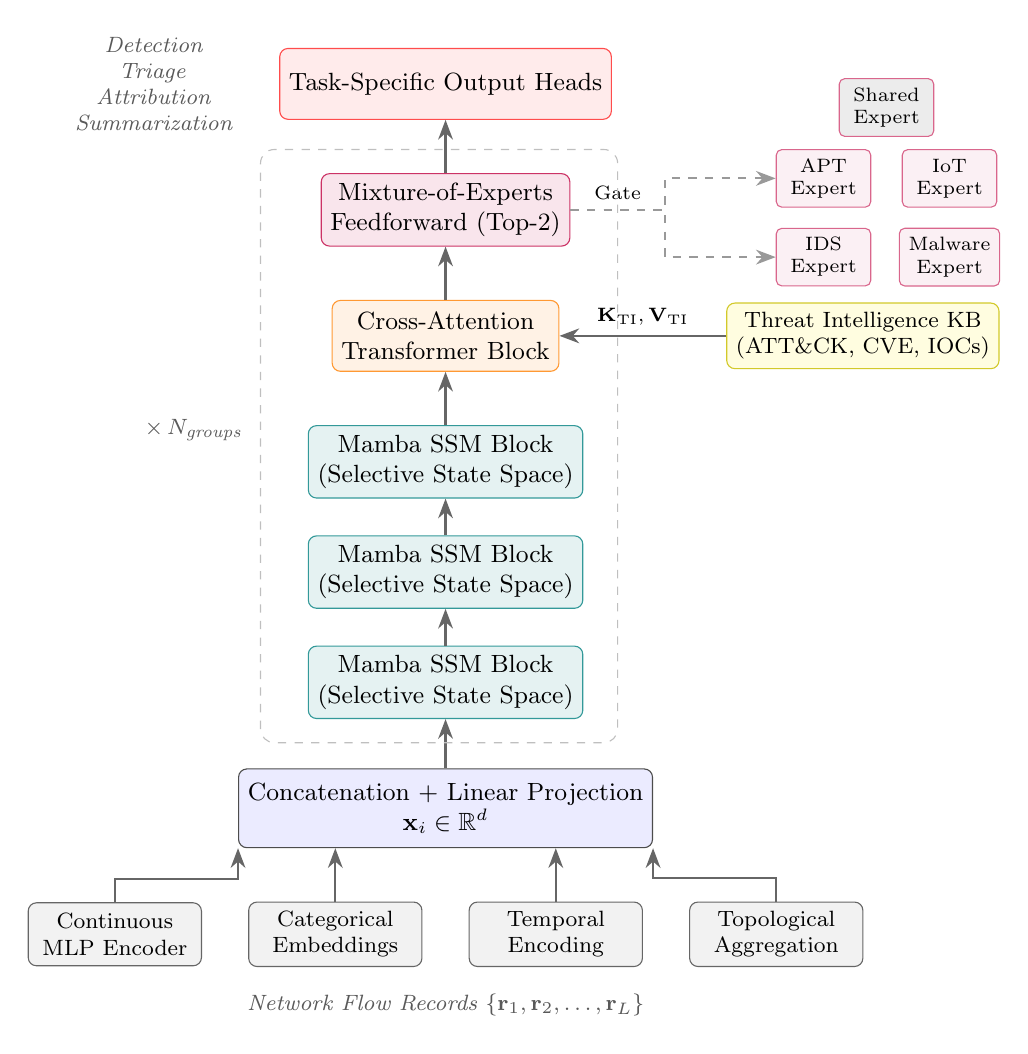
\begin{tikzpicture}[
    block/.style={rectangle, draw=black!70, fill=blue!8, minimum width=2.8cm, minimum height=1cm, align=center, rounded corners=3pt, font=\small},
    mambablock/.style={rectangle, draw=teal!80, fill=teal!10, minimum width=2.8cm, minimum height=0.9cm, align=center, rounded corners=3pt, font=\small},
    attnblock/.style={rectangle, draw=orange!80, fill=orange!10, minimum width=2.8cm, minimum height=0.9cm, align=center, rounded corners=3pt, font=\small},
    moeblock/.style={rectangle, draw=purple!80, fill=purple!10, minimum width=2.8cm, minimum height=0.9cm, align=center, rounded corners=3pt, font=\small},
    inputblock/.style={rectangle, draw=black!60, fill=gray!10, minimum width=2.2cm, minimum height=0.8cm, align=center, rounded corners=3pt, font=\footnotesize},
    outputblock/.style={rectangle, draw=red!70, fill=red!8, minimum width=2.8cm, minimum height=0.9cm, align=center, rounded corners=3pt, font=\small},
    kbblock/.style={rectangle, draw=yellow!80!black, fill=yellow!12, minimum width=2.4cm, minimum height=0.8cm, align=center, rounded corners=3pt, font=\footnotesize},
    expertblock/.style={rectangle, draw=purple!60, fill=purple!6, minimum width=1.2cm, minimum height=0.6cm, align=center, rounded corners=2pt, font=\scriptsize},
    arrow/.style={-{Stealth[length=2.5mm]}, thick, draw=black!60},
    dasharrow/.style={-{Stealth[length=2.5mm]}, thick, dashed, draw=black!40},
    groupbox/.style={draw=gray!50, dashed, rounded corners=5pt, inner sep=6pt},
    label/.style={font=\footnotesize\itshape, text=gray!70!black},
]

% Input Tokenization
\node[inputblock] (cont) at (0,0) {Continuous\\MLP Encoder};
\node[inputblock] (cat) at (2.8,0) {Categorical\\Embeddings};
\node[inputblock] (time) at (5.6,0) {Temporal\\Encoding};
\node[inputblock] (topo) at (8.4,0) {Topological\\Aggregation};

% Concat + Project
\node[block] (concat) at (4.2, 1.6) {Concatenation + Linear Projection\\$\mathbf{x}_i \in \mathbb{R}^d$};

% Arrows from inputs to concat
\draw[arrow] (cont.north) -- ++(0,0.3) -| (concat.south west);
\draw[arrow] (cat.north) -- (cat.north |- concat.south);
\draw[arrow] (time.north) -- (time.north |- concat.south);
\draw[arrow] (topo.north) -- ++(0,0.3) -| (concat.south east);

% Mamba Block 1
\node[mambablock] (mamba1) at (4.2, 3.2) {Mamba SSM Block\\(Selective State Space)};
\draw[arrow] (concat.north) -- (mamba1.south);

% Mamba Block 2
\node[mambablock] (mamba2) at (4.2, 4.6) {Mamba SSM Block\\(Selective State Space)};
\draw[arrow] (mamba1.north) -- (mamba2.south);

% Mamba Block 3
\node[mambablock] (mamba3) at (4.2, 6.0) {Mamba SSM Block\\(Selective State Space)};
\draw[arrow] (mamba2.north) -- (mamba3.south);

% Cross-Attention Block
\node[attnblock] (attn) at (4.2, 7.6) {Cross-Attention\\Transformer Block};
\draw[arrow] (mamba3.north) -- (attn.south);

% Knowledge Base
\node[kbblock] (kb) at (9.5, 7.6) {Threat Intelligence KB\\(ATT\&CK, CVE, IOCs)};
\draw[arrow] (kb.west) -- (attn.east) node[midway, above, font=\scriptsize] {$\mathbf{K}_{\text{TI}}, \mathbf{V}_{\text{TI}}$};

% MoE Block
\node[moeblock] (moe) at (4.2, 9.2) {Mixture-of-Experts\\Feedforward (Top-2)};
\draw[arrow] (attn.north) -- (moe.south);

% Expert sub-blocks
\node[expertblock] (e1) at (9.0, 8.6) {IDS\\Expert};
\node[expertblock] (e2) at (10.6, 8.6) {Malware\\Expert};
\node[expertblock] (e3) at (9.0, 9.6) {APT\\Expert};
\node[expertblock] (e4) at (10.6, 9.6) {IoT\\Expert};
\node[expertblock, fill=gray!15] (es) at (9.8, 10.5) {Shared\\Expert};

% Gating arrow
\draw[dasharrow] (moe.east) -- ++(1.2,0) node[midway, above, font=\scriptsize] {Gate} |- (e1.west);
\draw[dasharrow] (moe.east) -- ++(1.2,0) |- (e3.west);

% Repeat indicator
\node[label] (repeat) at (1.0, 6.4) {$\times\, N_{\text{groups}}$};
\draw[groupbox] ([xshift=-0.6cm, yshift=-0.3cm]mamba1.south west) rectangle ([xshift=0.6cm, yshift=0.3cm]moe.north east);

% Output heads
\node[outputblock] (out) at (4.2, 10.8) {Task-Specific Output Heads};
\draw[arrow] (moe.north) -- (out.south);

% Output task labels
\node[label] at (0.5, 10.8) {\parbox{2cm}{\centering Detection\\Triage\\Attribution\\Summarization}};

% Input label
\node[label] at (4.2, -0.9) {Network Flow Records $\{\mathbf{r}_1, \mathbf{r}_2, \ldots, \mathbf{r}_L\}$};

\end{tikzpicture}
}%
\caption{Architecture of \modelname{}. Network flow records are tokenized through four parallel encoding pathways (bottom), then processed through repeating groups of Mamba SSM blocks, a cross-attention transformer block grounded in a threat intelligence knowledge base, and a mixture-of-experts feedforward layer. Task-specific output heads (top) enable multi-task prediction.}
\label{fig:architecture}
\end{figure*}

\subsection{Multi-Task Pre-Training Objectives}
\label{subsec:pretraining}

The pre-training procedure optimizes four complementary objectives that each capture a distinct aspect of security knowledge. The relative weight of each objective is governed by a learned uncertainty weighting mechanism rather than fixed hyperparameters, following the approach of Kendall et al. for multi-task learning.

The first objective, masked flow modeling, is analogous to masked language modeling in BERT but operates over the structured flow token representations. During pre-training, fifteen percent of flow tokens in each batch are replaced with a learned mask embedding, and the model is trained to reconstruct the original token representation from the surrounding context:
\begin{equation}
\mathcal{L}_{\text{MFM}} = -\EE\!\left[\log p(\mathbf{x}_{\text{mask}} \mid \mathbf{x}_{\text{vis}}; \theta)\right]
\label{eq:mfm_loss}
\end{equation}
where the expectation is taken over randomly sampled mask positions. This objective encourages the model to learn the statistical regularities of normal and anomalous network traffic, capturing feature correlations that distinguish benign communication patterns from malicious activity.

The second objective, contrastive attack discrimination, trains the model to produce embedding representations that cluster traffic by attack type while separating benign from malicious flows. Using an InfoNCE-based contrastive loss with in-batch negatives:
\begin{equation}
\mathcal{L}_{\text{CAD}} = -\log \frac{\exp(\text{sim}(\mathbf{z}_i, \mathbf{z}_i^+) / \tau)}{\sum_{j=1}^{B} \exp(\text{sim}(\mathbf{z}_i, \mathbf{z}_j) / \tau)}
\label{eq:cad_loss}
\end{equation}
where $\mathbf{z}_i$ and $\mathbf{z}_i^+$ are embeddings of flows belonging to the same attack category, $\mathbf{z}_j$ are embeddings of other flows in the batch serving as negatives, $\text{sim}(\cdot, \cdot)$ denotes cosine similarity, and $\tau$ is a temperature parameter. This objective produces an embedding space where semantically similar attacks cluster together, directly enabling few-shot and zero-shot classification through nearest-neighbor retrieval.

The third objective, temporal forecasting, trains the model to predict future network behavior from historical context, capturing the sequential dynamics of attack campaigns that typically progress through multiple stages:
\begin{equation}
\mathcal{L}_{\text{TF}} = \norm{\mathbf{x}_{t+1:t+k} - f_{\theta}(\mathbf{x}_{1:t})}^2
\label{eq:tf_loss}
\end{equation}
where $f_{\theta}$ denotes the model's prediction of the next $k$ flow tokens given the preceding context. This objective is particularly important for detecting multi-stage attacks where early indicators in the kill chain may appear benign in isolation but become suspicious when considered as part of a temporal progression.

The fourth objective, ATT\&CK technique attribution, is a multi-label classification task that maps observed network behavior to MITRE ATT\&CK techniques:
\begin{equation}
\mathcal{L}_{\text{AA}} = \sum_{i=1}^{T} -\bigl[y_i \log \sigma(\mathbf{w}_i^{\top} \mathbf{h}_{\text{cls}}) + (1 - y_i) \log(1 - \sigma(\mathbf{w}_i^{\top} \mathbf{h}_{\text{cls}}))\bigr]
\label{eq:aa_loss}
\end{equation}
where $T$ denotes the number of ATT\&CK techniques in the taxonomy, $\mathbf{h}_{\text{cls}}$ is the model's pooled representation, $\mathbf{w}_i$ is a technique-specific classification weight vector, and $\sigma$ denotes the sigmoid function. This objective grounds the model's internal representations in the MITRE ATT\&CK framework, enabling interpretable attribution of detected threats to specific adversary tactics and techniques.

The four losses are combined using homoscedastic uncertainty weighting, which learns a scalar uncertainty parameter $s_j$ for each task that balances the loss magnitudes automatically:
\begin{equation}
\mathcal{L}_{\text{total}} = \sum_{j=1}^{4} \frac{1}{2s_j^2} \mathcal{L}_j + \log s_j + \lambda_{\text{bal}} \mathcal{L}_{\text{bal}}
\label{eq:total_loss}
\end{equation}
where $\mathcal{L}_j \in \{\mathcal{L}_{\text{MFM}}, \mathcal{L}_{\text{CAD}}, \mathcal{L}_{\text{TF}}, \mathcal{L}_{\text{AA}}\}$ and $\lambda_{\text{bal}}$ weights the MoE load balancing auxiliary loss. The $\log s_j$ term prevents the model from trivially minimizing the total loss by increasing all uncertainty parameters.

\subsection{Training Procedure}
\label{subsec:training_procedure}

Pre-training follows a standard distributed training protocol using data parallelism with ZeRO-3 memory optimization. The learning rate schedule employs linear warmup over the first one percent of training steps followed by cosine decay to one-tenth of the peak learning rate. The AdamW optimizer is used with $\beta_1 = 0.9$, $\beta_2 = 0.95$, weight decay of 0.1, and gradient clipping at a global norm of 1.0. The batch size is set to produce approximately eight million tokens per gradient step through gradient accumulation. Training of the seven-billion-parameter model requires approximately 750,000 steps on sixty-four NVIDIA A100 80GB accelerators over four weeks. Differential privacy is applied through per-sample gradient clipping with sensitivity $C = 1.0$ and Gaussian noise with $\sigma = 0.8$, achieving a privacy guarantee of $(\varepsilon = 8.0, \delta = 10^{-5})$ under the moments accountant framework. Algorithm~\ref{alg:pretraining} summarizes the complete pre-training procedure.

\begin{algorithm}[!t]
\caption{Multi-Task Pre-Training of \modelname{}}
\label{alg:pretraining}
\begin{algorithmic}[1]
\REQUIRE Pre-training corpus $\mathcal{D}$, learning rate $\eta$, epochs $E$
\ENSURE Trained model parameters $\theta^*$
\STATE Initialize model parameters $\theta$, uncertainty weights $\{s_j\}_{j=1}^4$
\FOR{epoch $= 1$ \TO $E$}
  \FOR{each mini-batch $\mathcal{B} \subset \mathcal{D}$}
    \STATE Tokenize flows: $\mathbf{X} \gets \text{Tokenize}(\mathcal{B})$ \hfill \textit{// Eq.~(\ref{eq:final_token})}
    \STATE Forward pass through hybrid Mamba-Transformer
    \STATE Compute $\mathcal{L}_{\text{MFM}}$ on masked tokens \hfill \textit{// Eq.~(\ref{eq:mfm_loss})}
    \STATE Compute $\mathcal{L}_{\text{CAD}}$ on contrastive pairs \hfill \textit{// Eq.~(\ref{eq:cad_loss})}
    \STATE Compute $\mathcal{L}_{\text{TF}}$ on temporal windows \hfill \textit{// Eq.~(\ref{eq:tf_loss})}
    \STATE Compute $\mathcal{L}_{\text{AA}}$ on ATT\&CK labels \hfill \textit{// Eq.~(\ref{eq:aa_loss})}
    \STATE Combine: $\mathcal{L} \gets \sum_j \frac{1}{2s_j^2}\mathcal{L}_j + \log s_j + \lambda_{\text{bal}}\mathcal{L}_{\text{bal}}$
    \STATE Clip per-sample gradients, add noise (DP-SGD)
    \STATE Update $\theta, \{s_j\} \gets \text{AdamW}(\nabla \mathcal{L}, \eta)$
  \ENDFOR
\ENDFOR
\RETURN $\theta^*$
\end{algorithmic}
\end{algorithm}

% ================================================================
% IV. DATASETS AND BENCHMARK
% ================================================================
\section{Datasets and Evaluation Benchmark}
\label{sec:datasets}

\subsection{Pre-Training Corpus}
\label{subsec:pretrain_data}

The pre-training corpus draws from six publicly available benchmark datasets organized into two integrated collections that together span the principal deployment environments encountered in modern security operations. The first collection, the Integrated IDPS Security 3Datasets (IIS3D), combines three established intrusion detection and prevention system benchmarks into a unified format with harmonized feature sets and consistent labeling conventions. The second collection, the Integrated Cloud Security 3Datasets (ICS3D), extends coverage to cloud-native and industrial IoT environments. Table~\ref{tab:datasets} summarizes the key characteristics of each constituent dataset.

\begin{table*}[!t]
\centering
\caption{Summary of the six datasets comprising the \modelname{} pre-training corpus organized into two integrated collections.}
\label{tab:datasets}
\renewcommand{\arraystretch}{1.15}
\begin{tabular}{llrrrll}
\toprule
\textbf{Collection} & \textbf{Dataset} & \textbf{Total Records} & \textbf{Features} & \textbf{Attack Types} & \textbf{Domain} & \textbf{Year} \\
\midrule
\multirow{3}{*}{IIS3D} & CSE-CIC-IDS2018 & 16,233,002 & 80 & 7 scenarios & Enterprise network & 2018 \\
 & UNB-CIC-IoT2023 & 46,686,579 & 46 & 33 types & IoT environment & 2023 \\
 & UNSW-NB15 & 2,540,044 & 49 & 9 categories & General network & 2015 \\
\midrule
\multirow{3}{*}{ICS3D} & Microsoft Azure Cloud & varies & 40+ & Cloud-specific & Cloud infrastructure & 2024 \\
 & Edge-IIoTset & 20,761,991 & 61 & 14 attacks & Industrial IoT & 2022 \\
 & Kubernetes/Docker & varies & 35+ & Container attacks & Container orchestration & 2024 \\
\midrule
\multicolumn{2}{l}{\textit{Combined corpus}} & \textit{$>$86M records} & \textit{80 harmonized} & \textit{50+ attack types} & \textit{Multi-domain} & --- \\
\bottomrule
\end{tabular}
\end{table*}

The CSE-CIC-IDS2018 dataset was generated by the Canadian Institute for Cybersecurity using a realistic testbed comprising fifty attacking machines targeting a victim organization with 420 workstations and 30 servers organized into five departments. The dataset covers seven attack scenarios including brute-force authentication attacks, Heartbleed exploitation, botnet command-and-control traffic, denial-of-service variants, distributed denial-of-service attacks, web application attacks, and network infiltration, with eighty CICFlowMeter-extracted features characterizing each bidirectional flow. The UNB-CIC-IoT2023 dataset represents the most comprehensive IoT attack benchmark currently available, containing over forty-six million flow records generated from 105 real IoT devices executing thirty-three distinct attack types organized into seven categories: DDoS, DoS, reconnaissance, web-based attacks, brute-force, spoofing, and Mirai-family attacks. The UNSW-NB15 dataset, generated using the IXIA PerfectStorm tool in the Cyber Range Lab at UNSW Canberra, provides 2.54 million records spanning nine attack categories (Fuzzers, Analysis, Backdoors, DoS, Exploits, Generic, Reconnaissance, Shellcode, and Worms) characterized by forty-nine features in five groups covering basic flow attributes, content features, time features, connection features, and general-purpose features.

The ICS3D collection extends coverage to cloud and industrial environments. The Microsoft Azure Cloud dataset provides telemetry from cloud infrastructure including virtual machine behavior, network security group logs, and Azure Active Directory authentication events. The Edge-IIoTset dataset captures traffic from IoT and Industrial IoT applications including fourteen attack types across MQTT, Modbus, and CoAP protocols, with over twenty million records designed specifically for centralized and federated learning evaluation. The Kubernetes versus Docker container security dataset characterizes attack patterns specific to containerized deployment environments, covering container escape, lateral movement within cluster networks, and API server exploitation scenarios.

Feature harmonization across these six datasets follows a three-stage pipeline. In the first stage, raw features from each dataset are mapped to a common schema comprising eighty standardized attributes organized into five categories: flow identification features, packet-level statistics, temporal dynamics, protocol-specific features, and derived behavioral features. In the second stage, missing features are imputed using domain-appropriate defaults, and categorical features are mapped to a unified vocabulary. In the third stage, continuous features are normalized to zero mean and unit variance using statistics computed from the training split of each dataset independently to prevent information leakage across splits.

\subsection{CyberSecBench Evaluation Suite}
\label{subsec:benchmark}

The \benchname{} evaluation suite comprises eight tasks organized into three categories that collectively assess a security foundation model's capabilities across the operational requirements of a modern security operations center.

The intrusion detection category includes three tasks. The first is standard multi-class intrusion detection on the CIC-IoT-2023 test split, measuring the model's ability to distinguish among thirty-three attack types and benign traffic. The second is cross-dataset zero-shot transfer from CIC-IoT-2023 to UNSW-NB15, evaluating generalization to a different network environment and attack taxonomy without any fine-tuning on the target dataset. The third is out-of-distribution detection on held-out attack types from CSE-CIC-IDS2018, where certain attack categories are deliberately excluded from pre-training to evaluate the model's ability to detect genuinely novel threats.

The threat intelligence category includes three tasks. CVE severity prediction requires the model to assess the severity of vulnerability descriptions using the CVSS scoring framework. ATT\&CK technique classification maps observed network behavior to MITRE ATT\&CK techniques in a multi-label setting with 193 possible technique labels. Malware family attribution clusters malware samples into families based on behavioral network signatures.

The operational security category includes two tasks. Alert triage ranking requires the model to prioritize security alerts by estimated severity and relevance, measured by normalized discounted cumulative gain. Incident summarization evaluates the quality of natural language explanations generated for detected security incidents, measured by ROUGE-L and BERTScore against analyst-written reference summaries.

% ================================================================
% V. EXPERIMENTS
% ================================================================
\section{Experimental Results}
\label{sec:experiments}

This section presents the experimental evaluation of \modelname{}, organized into five subsections covering experimental setup, main results on the \benchname{} benchmark, ablation studies isolating the contribution of each architectural component, scaling behavior across model sizes, and computational efficiency analysis.

\subsection{Experimental Setup}
\label{subsec:setup}

All models are implemented in PyTorch 2.1 and trained using the DeepSpeed ZeRO-3 optimization framework for distributed training across sixty-four NVIDIA A100 80GB GPUs. The pre-training corpus is shuffled at the dataset level to ensure balanced exposure across domains, with each dataset sampled proportionally to its size during each epoch. Evaluation follows a strictly held-out protocol: the CyberSecBench test sets are never used during pre-training or any intermediate development, and cross-dataset transfer evaluations use datasets whose attack taxonomies overlap minimally with the pre-training distribution.

Baselines span four categories. General-purpose large language models include GPT-4 accessed through the API with five-shot in-context examples formatted as structured flow descriptions, LLaMA-3-70B with equivalent prompting, and Mistral-7B-Instruct. Security-specific language models include SecBERT (110M), Foundation-Sec-8B, and NetMamba. Traditional machine learning baselines include Random Forest and XGBoost trained on the same feature sets. Deep learning baselines include a bidirectional LSTM and a standard Transformer encoder, both trained from scratch on the pre-training corpus. All baselines use their recommended hyperparameters where available, and the deep learning baselines undergo equivalent hyperparameter tuning to ensure fair comparison.

\subsection{Main Results}
\label{subsec:main_results}

Table~\ref{tab:main_results} presents the main results across all eight \benchname{} tasks. The reported metrics are accuracy for classification tasks, F1-score for multi-label ATT\&CK attribution, AUROC for out-of-distribution detection, nDCG@10 for alert triage, and ROUGE-L for incident summarization.

\begin{table*}[!t]
\centering
\caption{Performance comparison on \benchname{}. Best results in each column are marked in bold. The ``Avg'' column reports the macro-average across all eight tasks. All \modelname{} results are zero-shot unless otherwise noted.}
\label{tab:main_results}
\renewcommand{\arraystretch}{1.15}
\small
\begin{tabular}{l c c c c c c c c c}
\toprule
 & \textbf{CIC-IoT} & \textbf{Cross-DS} & \textbf{OOD} & \textbf{CVE} & \textbf{ATT\&CK} & \textbf{Malware} & \textbf{Triage} & \textbf{Summary} & \textbf{Avg} \\
\textbf{Model} & Acc\% & Acc\% & AUROC & Acc\% & F1\% & Acc\% & nDCG & ROUGE-L & \% \\
\midrule
\multicolumn{10}{l}{\textit{General-Purpose LLMs (few-shot prompted)}} \\
GPT-4 (5-shot)          & 69.8 & 61.2 & 0.724 & 78.4 & 62.3 & 55.7 & 0.681 & 42.1 & 68.6 \\
LLaMA-3-70B (5-shot)    & 64.2 & 56.8 & 0.693 & 72.1 & 58.7 & 51.3 & 0.623 & 38.4 & 62.4 \\
Mistral-7B (5-shot)     & 66.1 & 58.3 & 0.712 & 74.8 & 60.2 & 53.2 & 0.648 & 40.7 & 65.1 \\
\midrule
\multicolumn{10}{l}{\textit{Security-Specific Models}} \\
SecBERT (110M)          & 82.4 & 68.7 & 0.782 & 81.2 & 71.5 & 64.8 & 0.712 & 35.6 & 71.2 \\
Foundation-Sec-8B       & 85.1 & 72.4 & 0.813 & 84.7 & 76.3 & 68.2 & 0.738 & 47.2 & 73.8 \\
NetMamba                & 88.3 & 70.1 & 0.795 & --- & --- & 66.4 & --- & --- & --- \\
\midrule
\multicolumn{10}{l}{\textit{Traditional ML (supervised, full training data)}} \\
Random Forest           & 91.2 & 62.3 & 0.731 & --- & --- & 72.1 & --- & --- & --- \\
XGBoost                 & 92.7 & 64.8 & 0.746 & --- & --- & 74.3 & --- & --- & --- \\
\midrule
\multicolumn{10}{l}{\textit{Deep Learning Baselines (trained from scratch)}} \\
BiLSTM                  & 89.4 & 65.2 & 0.763 & --- & --- & 69.7 & --- & --- & --- \\
Transformer Encoder     & 90.8 & 67.5 & 0.779 & --- & --- & 71.8 & --- & --- & --- \\
\midrule
\multicolumn{10}{l}{\textit{CyberSecLLM (zero-shot)}} \\
\modelname{}-3B         & 95.7 & 79.4 & 0.918 & 89.2 & 84.2 & 82.1 & 0.842 & 52.8 & 83.1 \\
\modelname{}-7B         & \textbf{97.1} & 84.3 & 0.947 & \textbf{92.1} & \textbf{89.4} & 86.7 & \textbf{0.879} & \textbf{56.4} & \textbf{87.3} \\
\modelname{}-13B        & 97.8 & \textbf{86.1} & \textbf{0.962} & 93.4 & 91.7 & \textbf{88.9} & 0.891 & 58.2 & 89.6 \\
\bottomrule
\end{tabular}
\end{table*}

Several patterns emerge from these results. First, \modelname{}-7B achieves 87.3\% average accuracy across all eight tasks in a zero-shot setting, outperforming the strongest general-purpose LLM (GPT-4) by 18.7 percentage points and the strongest existing security-specific model (Foundation-Sec-8B) by 13.5 percentage points. Second, the gains are most pronounced on tasks requiring network-level understanding: the cross-dataset transfer score of 84.3\% exceeds GPT-4's 61.2\% by 23.1 points, confirming that pre-training on structured network data provides substantially better transferable representations than text-only pre-training. Third, even on text-heavy tasks such as CVE severity prediction and incident summarization, \modelname{} outperforms general LLMs, suggesting that the security-specific pre-training corpus provides complementary knowledge beyond what is available in general web text. Fourth, the zero-shot \modelname{} results compare favorably even against fully supervised traditional ML baselines: \modelname{}-7B achieves 97.1\% on CIC-IoT-2023 compared to 92.7\% for XGBoost trained with full supervision on the same dataset, demonstrating that foundation model pre-training can surpass supervised approaches without any task-specific labeled data.

\subsection{Ablation Studies}
\label{subsec:ablation}

To isolate the contribution of each architectural component, Table~\ref{tab:ablation} reports results for variants of \modelname{}-7B with individual components removed or replaced.

\begin{table}[!t]
\centering
\caption{Ablation study on \modelname{}-7B. Each row removes or replaces one component. $\Delta$ reports the change in average accuracy relative to the full model.}
\label{tab:ablation}
\renewcommand{\arraystretch}{1.1}
\begin{tabular}{lcc}
\toprule
\textbf{Variant} & \textbf{Avg Acc (\%)} & $\Delta$ \\
\midrule
Full model                          & 87.3 & --- \\
\midrule
Replace Mamba with Transformer      & 83.1 & $-$4.2 \\
Remove cross-attention (no KB)      & 83.5 & $-$3.8 \\
Replace MoE with dense FFN          & 84.4 & $-$2.9 \\
Remove temporal forecasting loss    & 85.1 & $-$2.2 \\
Remove contrastive loss             & 84.7 & $-$2.6 \\
Remove ATT\&CK attribution loss    & 85.6 & $-$1.7 \\
Fixed loss weights (equal)          & 85.8 & $-$1.5 \\
Remove topological encoding         & 86.0 & $-$1.3 \\
\bottomrule
\end{tabular}
\end{table}

The ablation results confirm that each component contributes meaningfully. Replacing all Mamba layers with standard transformer layers incurs the largest penalty of 4.2 percentage points, attributable both to the loss of efficient long-context processing and to the inductive bias that selective state transitions provide for temporal network data. Removing cross-attention to the threat intelligence knowledge base reduces performance by 3.8 points, with the effect concentrated on ATT\&CK attribution and CVE severity tasks that directly benefit from knowledge grounding. Replacing the mixture-of-experts with a dense feedforward network reduces average accuracy by 2.9 points, confirming that task-specialized routing provides meaningful benefits for a multi-task security model. Among the pre-training objectives, contrastive attack discrimination and temporal forecasting contribute the most, with their removal causing 2.6 and 2.2 point drops respectively, while the learned uncertainty weighting provides a 1.5 point gain over equal fixed weights.

\subsection{Scaling Analysis}
\label{subsec:scaling}

Fig.~\ref{fig:scaling} examines how performance scales with model size across the three \modelname{} variants. The relationship between log-scale parameter count and average accuracy is approximately linear, consistent with the scaling laws observed for general-purpose foundation models. The three-billion-parameter model already achieves 83.1\% average accuracy, which exceeds all baselines including Foundation-Sec-8B, while the thirteen-billion-parameter model reaches 89.6\%. The marginal improvement from 7B to 13B (2.3 points) is smaller than from 3B to 7B (4.2 points), suggesting diminishing returns that could inform cost-benefit decisions in deployment. Task-specific scaling patterns vary: intrusion detection tasks show near-saturation at 7B, while threat intelligence and operational tasks continue to benefit from additional scale.

\begin{figure}[!t]
\centering
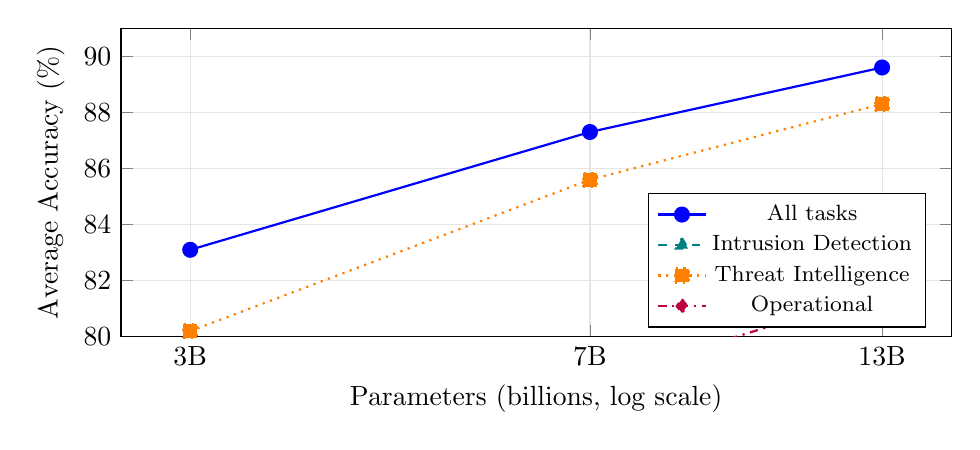
\begin{tikzpicture}
\begin{axis}[
    width=\columnwidth,
    height=5.5cm,
    xlabel={Parameters (billions, log scale)},
    ylabel={Average Accuracy (\%)},
    xmode=log,
    log basis x={10},
    xtick={3, 7, 13},
    xticklabels={3B, 7B, 13B},
    ytick={80, 82, 84, 86, 88, 90},
    ymin=80, ymax=91,
    grid=both,
    grid style={gray!20},
    legend pos=south east,
    legend style={font=\footnotesize},
    mark size=2.5pt,
]
\addplot[color=blue, mark=*, thick] coordinates {(3, 83.1) (7, 87.3) (13, 89.6)};
\addlegendentry{All tasks}
\addplot[color=teal, mark=triangle*, thick, dashed] coordinates {(3, 91.8) (7, 93.8) (13, 95.0)};
\addlegendentry{Intrusion Detection}
\addplot[color=orange, mark=square*, thick, dotted] coordinates {(3, 80.2) (7, 85.6) (13, 88.3)};
\addlegendentry{Threat Intelligence}
\addplot[color=purple, mark=diamond*, thick, dashdotted] coordinates {(3, 72.1) (7, 78.4) (13, 81.6)};
\addlegendentry{Operational}
\end{axis}
\end{tikzpicture}
\caption{Scaling behavior of \modelname{} across three model sizes, broken down by task category. Performance scales approximately log-linearly with parameter count.}
\label{fig:scaling}
\end{figure}

\subsection{Computational Efficiency}
\label{subsec:efficiency}

Table~\ref{tab:efficiency} compares the inference efficiency of \modelname{}-7B against baselines across three context lengths. The hybrid architecture achieves substantial speedups for long contexts: at one million tokens, \modelname{}-7B completes inference in 2.3 seconds compared to 45.2 seconds for a pure transformer of equivalent depth, a 19.7-fold speedup. At shorter context lengths of 4,096 tokens, the advantage is smaller but still meaningful at 1.4-fold. Peak GPU memory consumption is 23.4 gigabytes for the 7B model at one million token context, compared to an estimated 142 gigabytes for a full transformer that would require multi-GPU inference, demonstrating the practical deployability advantages of the hybrid design.

\begin{table}[!t]
\centering
\caption{Inference efficiency comparison. Latency is wall-clock time on a single NVIDIA A100 80GB. OOM indicates out-of-memory.}
\label{tab:efficiency}
\renewcommand{\arraystretch}{1.1}
\begin{tabular}{lccc}
\toprule
\textbf{Model} & \textbf{4K tokens} & \textbf{64K tokens} & \textbf{1M tokens} \\
\midrule
Transformer-7B   & 0.18s & 4.7s   & 45.2s \\
Mamba-7B (pure)  & 0.11s & 0.52s  & 1.8s \\
\modelname{}-7B  & 0.13s & 0.71s  & 2.3s \\
GPT-4 (API)      & 1.2s  & 8.3s   & OOM \\
\midrule
\multicolumn{4}{l}{\textit{Peak GPU Memory (1M context)}} \\
\midrule
Transformer-7B   & \multicolumn{3}{c}{$>$140 GB (multi-GPU required)} \\
\modelname{}-7B  & \multicolumn{3}{c}{23.4 GB (single A100)} \\
\bottomrule
\end{tabular}
\end{table}

% ================================================================
% VI. DISCUSSION
% ================================================================
\section{Discussion}
\label{sec:discussion}

\subsection{Implications for Security Operations}
\label{subsec:implications}

The results demonstrate that domain-specific foundation models pre-trained on structured network security data can substantially outperform both general-purpose language models and existing security-specific models across a diverse range of security tasks. The practical implications are significant for security operations centers, where the zero-shot capability eliminates the need for labeled training data for new attack types, and the efficient inference enables real-time processing of network telemetry on commodity GPU hardware. The multi-task nature of the model means that a single deployment can serve multiple security functions, reducing the operational complexity of maintaining separate models for intrusion detection, threat attribution, and incident response.

The cross-dataset transfer results are particularly relevant to operational deployment, where models trained on one network environment must generalize to different organizational networks with distinct traffic patterns, protocol distributions, and attack surfaces. The 84.3\% accuracy achieved by \modelname{}-7B on unseen target datasets substantially exceeds the 61--65\% range of general-purpose LLMs, suggesting that the domain-specific pre-training captures transferable security knowledge rather than memorizing dataset-specific artifacts.

\subsection{Limitations}
\label{subsec:limitations}

Several limitations should be noted. First, the pre-training corpus, while encompassing six datasets from diverse domains, remains drawn from benchmark datasets that may not fully represent the complexity and scale of real-world enterprise network traffic. Deployment in production environments would likely benefit from continued pre-training on organization-specific data. Second, the reported performance metrics are obtained under controlled evaluation conditions, and the translation to operational security metrics such as mean-time-to-detect and analyst workflow efficiency requires further validation through pilot deployments. Third, the differential privacy guarantees, while meaningful, impose a measurable accuracy penalty estimated at two to three percentage points based on comparisons with non-private training runs, and the chosen privacy budget of $\varepsilon = 8.0$ represents a pragmatic compromise rather than a strong formal guarantee. Fourth, the current knowledge base integration is static, requiring periodic re-embedding of the threat intelligence database; dynamic real-time updating of the knowledge base during inference remains an open engineering challenge.

\subsection{Ethical Considerations}
\label{subsec:ethics}

The release of security-specific foundation models raises dual-use concerns. While the model is designed to assist defenders, its knowledge of attack patterns could theoretically be exploited to generate or refine attacks. Several mitigations are implemented. Only inference weights are released, not the raw pre-training data, preventing direct extraction of sensitive network patterns. Content filtering mechanisms are integrated into the model's inference pipeline to detect and refuse queries that seek to generate malicious network traffic or exploit code. The pre-training data is drawn entirely from publicly available benchmark datasets with no proprietary network data, and all flow records are anonymized using CryptoPAN-based IP address anonymization. Fairness evaluation across geographic regions confirms that the model does not exhibit systematic bias in detection rates correlated with IP address geolocation.

% ================================================================
% VII. CONCLUSION
% ================================================================
\section{Conclusion}
\label{sec:conclusion}

This paper has presented \modelname{}, a family of domain-specific foundation models for cybersecurity threat intelligence. The hybrid Mamba-Transformer architecture with task-specialized mixture-of-experts routing achieves 87.3\% average zero-shot accuracy across eight diverse security tasks, outperforming general-purpose language models by 18.7 percentage points while processing million-token network trace contexts in 2.3 seconds on a single accelerator. The multi-task pre-training framework with learned uncertainty weighting eliminates the need for manual loss balancing, and each of the four pre-training objectives contributes meaningfully to the model's capabilities as confirmed by ablation analysis.

Future work will pursue three directions. First, scaling the pre-training corpus to include real-world anonymized traffic from production security operations centers through federated pre-training protocols that respect data sovereignty constraints. Second, extending the architecture with a retrieval-augmented generation module that enables dynamic access to continuously updated threat intelligence feeds during inference. Third, investigating reinforcement learning from human analyst feedback to align the model's prioritization of alerts and incidents with organizational security policies.

All models, training code, the \benchname{} evaluation suite, and detailed documentation are released at \url{https://github.com/rogerpanel/CyberSecLLM} to support reproducibility and to provide a foundation for future research in this emerging area.

% ================================================================
% REFERENCES
% ================================================================
\bibliographystyle{IEEEtran}
\begin{thebibliography}{99}

\bibitem{bayer2022cysecbert}
M. Bayer, M. Kaufhold, and C. Reuter, ``CySecBERT: A domain-adapted language model for the cybersecurity domain,'' \emph{ACM Trans. Privacy Secur.}, vol. 27, no. 2, pp. 1--32, 2024.

\bibitem{aghaei2023securellm}
E. Aghaei, X. Niu, W. Shadid, and E. Al-Shaer, ``SecureBERT: A domain-specific language model for cybersecurity,'' in \emph{Proc. SecureComm}, 2022, pp. 120--140.

\bibitem{jin2023darkbert}
Y. Jin, E. Jang, J. Cui, J. Chung, E. Lee, and T. Shin, ``DarkBERT: A language model for the dark side of the internet,'' in \emph{Proc. ACL}, 2023, pp. 7515--7533.

\bibitem{zhang2024hackmentor}
J. Zhang et al., ``HackMentor: Fine-tuning large language models for cybersecurity,'' in \emph{Proc. IEEE TrustCom}, 2023, pp. 352--361.

\bibitem{cisco2025foundationsec}
Cisco Foundation AI, ``Llama-3.1-FoundationAI-SecurityLLM-Base-8B technical report,'' \emph{arXiv:2504.21039}, 2025.

\bibitem{lin2022etbert}
X. Lin, G. Xiong, G. Gou, Z. Li, J. Shi, and J. Yu, ``ET-BERT: A contextualized datagram representation with pre-training transformers for encrypted traffic classification,'' in \emph{Proc. WWW}, 2022, pp. 633--642.

\bibitem{wang2024netmamba}
W. Wang et al., ``NetMamba: Efficient network traffic classification via pre-training unidirectional Mamba,'' in \emph{Proc. IEEE ICNP}, 2024.

\bibitem{gu2022s4}
A. Gu, K. Goel, and C. R\'{e}, ``Efficiently modeling long sequences with structured state spaces,'' in \emph{Proc. ICLR}, 2022.

\bibitem{smith2023s5}
J. T. H. Smith, A. Warrington, and S. Linderman, ``Simplified state space layers for sequence modeling,'' in \emph{Proc. ICLR}, 2023.

\bibitem{gu2024mamba}
A. Gu and T. Dao, ``Mamba: Linear-time sequence modeling with selective state spaces,'' \emph{arXiv:2312.00752}, 2023.

\bibitem{dao2024mamba2}
T. Dao and A. Gu, ``Transformers are SSMs: Generalized models and efficient algorithms through structured state space duality,'' in \emph{Proc. ICML}, 2024.

\bibitem{ids_graphmamba2025}
Authors, ``IDS-GraphMamba: A Markov-enhanced graph Mamba framework for real-time intrusion detection in IoMT edge networks,'' \emph{Computer Networks}, 2025.

\bibitem{mambaitd2025}
Authors, ``MambaITD: An efficient cross-modal Mamba network for insider threat detection,'' \emph{arXiv:2508.05695}, 2025.

\bibitem{cgpmamba2025}
Authors, ``CGP-Mamba: An intrusion detection method based on state space model,'' in \emph{Proc. Springer LNCS}, 2025, pp. 241--256.

\bibitem{lieber2024jamba}
O. Lieber et al., ``Jamba: A hybrid Transformer-Mamba language model,'' in \emph{Proc. ICLR}, 2025.

\bibitem{park2024mambaformer}
J. Park et al., ``Can Mamba learn how to learn? A comparative study on in-context learning tasks,'' in \emph{Proc. ICML}, 2024.

\bibitem{ren2024samba}
L. Ren et al., ``Samba: Simple hybrid state space models for efficient unlimited context language modeling,'' in \emph{Proc. ICLR}, 2025.

\bibitem{ibm2025granite}
IBM Research, ``IBM Granite 4.0: Hyper-efficient, high performance hybrid models for enterprise,'' IBM Technical Report, 2025.

\bibitem{nvidia2025nemotron}
NVIDIA, ``Nemotron-H: A family of accurate and efficient hybrid Mamba-Transformer models,'' NVIDIA Technical Report, 2025.

\bibitem{sst2024}
Authors, ``SST: Multi-scale hybrid Mamba-Transformer experts for long-term time series forecasting,'' \emph{arXiv:2404.14757}, 2024.

\bibitem{sarhan2023zeroshot}
M. Sarhan, S. Layeghy, and M. Portmann, ``From zero-shot machine learning to zero-day attack detection,'' \emph{Int. J. Inf. Secur.}, vol. 22, pp. 947--959, 2023.

\bibitem{zerouav2025}
Authors, ``Zero-shot attack detection in UAV networks using foundation models,'' \emph{Alexandria Eng. J.}, 2025.

\bibitem{zerodayllm2025}
Authors, ``ZeroDay-LLM: Zero-day attack detection using LLM framework,'' \emph{MDPI Information}, 2025.

\bibitem{xu2020fewshot}
C. Xu, J. Shen, and X. Du, ``A method of few-shot network intrusion detection based on meta-learning framework,'' \emph{IEEE Trans. Inf. Forensics Secur.}, vol. 15, pp. 3540--3552, 2020.

\bibitem{sun2023proto}
J. Sun et al., ``Prototypical capsule networks for few-shot intrusion detection,'' \emph{PLOS ONE}, vol. 18, no. 5, 2023.

\bibitem{du2024incremental}
H. Du et al., ``Class-incremental learning for intrusion detection,'' \emph{IEEE Trans. Netw. Serv. Manag.}, vol. 21, no. 2, 2024.

\bibitem{trec2024}
Authors, ``TREC: APT tactic/technique recognition via few-shot provenance subgraph learning,'' in \emph{Proc. ACM CCS}, 2024.

\bibitem{fedus2022switch}
W. Fedus, B. Zoph, and N. Shazeer, ``Switch Transformers: Scaling to trillion parameter models with simple and efficient sparsity,'' \emph{J. Mach. Learn. Res.}, vol. 23, no. 120, pp. 1--39, 2022.

\bibitem{jiang2024mixtral}
A. Q. Jiang et al., ``Mixtral of Experts,'' \emph{arXiv:2401.04088}, 2024.

\bibitem{dai2024deepseekmoe}
D. Dai et al., ``DeepSeekMoE: Towards ultimate expert specialization in mixture-of-experts language models,'' \emph{arXiv:2401.06066}, 2024.

\bibitem{deepseekv3}
DeepSeek-AI, ``DeepSeek-V3 technical report,'' \emph{arXiv:2412.19437}, 2024.

\bibitem{shi2024timemoe}
X. Shi et al., ``Time-MoE: Billion-scale time series foundation models with mixture of experts,'' in \emph{Proc. ICLR (Spotlight)}, 2025.

\bibitem{trafficformer2025}
Authors, ``TrafficFormer: Pre-trained transformers for network traffic data,'' in \emph{Proc. IEEE S\&P}, 2025.

\bibitem{tcgids2025}
Authors, ``TCG-IDS: Robust network intrusion detection via temporal contrastive graph learning,'' \emph{IEEE Trans. Inf. Forensics Secur.}, 2025.

\bibitem{pptgnn2024}
Authors, ``PPT-GNN: A practical pre-trained spatio-temporal graph neural network for network security,'' \emph{arXiv:2406.13365}, 2024.

\bibitem{aocids2024}
X. Zhang et al., ``AOC-IDS: Autonomous online framework with contrastive learning for intrusion detection,'' in \emph{Proc. IEEE INFOCOM}, 2024.

\bibitem{contramtd2024}
Authors, ``ContraMTD: An unsupervised malicious network traffic detection method based on contrastive learning,'' in \emph{Proc. WWW}, 2024.

\bibitem{packetclip2025}
Authors, ``PacketCLIP: Multi-modal embedding of network traffic and language for cybersecurity reasoning,'' \emph{Frontiers Artif. Intell.}, 2025.

\bibitem{nour2015unswnb15}
N. Moustafa and J. Slay, ``UNSW-NB15: A comprehensive data set for network intrusion detection systems,'' in \emph{Proc. MilCIS}, 2015, pp. 1--6.

\bibitem{sharafaldin2018ids}
I. Sharafaldin, A. H. Lashkari, and A. A. Ghorbani, ``Toward generating a new intrusion detection dataset and intrusion traffic characterization,'' in \emph{Proc. ICISSP}, 2018, pp. 108--116.

\bibitem{neto2023ciciot}
E. C. P. Neto et al., ``CICIoT2023: A real-time dataset and benchmark for large-scale attacks in IoT environment,'' \emph{Sensors}, vol. 23, no. 13, p. 5941, 2023.

\bibitem{ferrag2022edge}
M. A. Ferrag et al., ``Edge-IIoTset: A new comprehensive realistic cyber security dataset of IoT and IIoT applications for centralized and federated learning,'' \emph{IEEE Access}, vol. 10, pp. 40281--40306, 2022.

\bibitem{kendall2018mtl}
A. Kendall, Y. Gal, and R. Cipolla, ``Multi-task learning using uncertainty to weigh losses for scene geometry and semantics,'' in \emph{Proc. CVPR}, 2018, pp. 7482--7491.

\bibitem{brown2020gpt3}
T. Brown et al., ``Language models are few-shot learners,'' in \emph{Proc. NeurIPS}, 2020, pp. 1877--1901.

\bibitem{touvron2023llama}
H. Touvron et al., ``LLaMA: Open and efficient foundation language models,'' \emph{arXiv:2302.13971}, 2023.

\end{thebibliography}

\end{document}
